\documentclass[11pt]{article}

\usepackage[utf8]{inputenc}
\usepackage[T1]{fontenc}
\usepackage{lmodern}
\usepackage[margin=1in]{geometry}
\usepackage{amsmath,amssymb}
\usepackage{graphicx}
\usepackage{booktabs}
\usepackage{siunitx}
\usepackage{verbatim}
\usepackage{caption}
\usepackage{subcaption}
\usepackage{xcolor}
\usepackage[colorlinks=true,linkcolor=blue,citecolor=blue,urlcolor=blue]{hyperref}

\graphicspath{{../results/figures/}{results/figures/}}

\title{\textbf{Machine Learning for BB84 Eavesdropping Detection\\
\large Technical Report and Project Status}}
\author{Yash Yadav \\ \small Indian Institute of Technology Kanpur}
\date{\today}

\begin{document}
\maketitle

\begin{abstract}
This is a complete technical record of the project: the BB84 quantum-channel
simulator and its physics, every attack model, the datasets and feature sets, the
classical / quantum / deep-learning detectors, the evaluation methodology, and all
results obtained so far. It is meant as a self-contained reference --- read it to
understand exactly what has been built, what each number means, and where the
project currently stands, including the adversarial-robustness study. Section
\ref{sec:status} gives an honest assessment of novelty.
\end{abstract}

\tableofcontents

\section{Overview and motivation}
The BB84 protocol certifies key security with a single statistic: if the quantum
bit error rate (QBER) exceeds $\sim$11\%, the key is discarded. This project asks
whether machine learning on \emph{richer} channel statistics can detect
eavesdropping that this threshold misses, and characterises three regimes:
\begin{enumerate}
  \item \textbf{Sub-threshold attacks} that hold QBER below 11\% but perturb other
  observables (per-basis QBER, decoy gains).
  \item \textbf{Quantum vs classical detectors}, including a quantum-kernel SVM and
  its failure mode (kernel concentration).
  \item \textbf{Temporally-structured attacks} whose aggregate statistics match a
  benign channel but whose error \emph{sequence} is clustered in time.
\end{enumerate}

\section{Physics background}
\paragraph{BB84.} Alice sends qubits prepared in a random bit and a random basis
($Z=\{\ket{0},\ket{1}\}$ or $X=\{\ket{+},\ket{-}\}$). Bob measures in a random
basis. After public \emph{sifting} (keeping events where their bases match), the
disagreement fraction is the QBER, which upper-bounds an eavesdropper's
information.

\paragraph{Intercept--resend and the threshold.} If Eve measures every qubit in a
random basis and resends, she is in the wrong basis half the time, each such event
giving a 25\% error: a full attack yields QBER $\approx 25\%$, far above 11\%.

\paragraph{Weak coherent pulses, loss, and decoy states.} Real sources emit
phase-randomised weak coherent pulses with photon number $k\sim\mathrm{Poisson}(\mu)$.
With channel transmittance $\eta$, the probability that Bob detects a pulse (its
\emph{gain}) is
\begin{equation}
  Q_\mu \;=\; \mathbb{E}_k\!\left[\,1-(1-\eta)^k\,\right] \;=\; 1 - e^{-\mu\eta}.
  \label{eq:gain}
\end{equation}
Sending two intensities --- a \emph{signal} $\mu_s$ and a weaker \emph{decoy}
$\mu_d$ --- lets Alice and Bob check that the per-intensity gains are mutually
consistent; this is what catches photon-number-splitting (Sec.~\ref{sec:pns}).

\section{Simulator: physics and algorithms}
The simulator (\texttt{src/bb84/simulator.py}) combines a real single-qubit
Qiskit-Aer circuit (for the quantum-mechanical error process) with a Monte-Carlo
photon/decoy layer (for loss, intensities, and PNS).

\subsection{Qubit preparation and measurement}
For one pulse with bit $b$, preparation basis $a$, and Bob basis $m$:
\begin{verbatim}
  qc = QuantumCircuit(1,1)
  if b == 1:      qc.x(0)      # set bit value first ...
  if a == 'X':    qc.h(0)      # ... then rotate into the basis
  if m == 'X':    qc.h(0)      # Bob's basis change
  qc.measure(0,0)
\end{verbatim}
The order matters: applying $H$ before $X$ would mis-prepare the X-basis bit-1
state ($\ket{-}$), which is a bug we found and fixed early --- it had injected a
spurious $\sim$25\% baseline QBER.

\subsection{Channel noise}
Channel noise is a depolarizing error of rate $\lambda$ (default $0.03$) applied to
the \texttt{h}, \texttt{x}, \texttt{z} gates via Qiskit-Aer's noise model. With no
attack and no noise the QBER is exactly $0$; at $\lambda=0.03$ the secure QBER is
$\approx 0.02$ (Table~\ref{tab:theory}).

\subsection{Photon / decoy channel model}
Each pulse is independently a signal ($\mu_s=0.5$) or decoy ($\mu_d=0.1$) with
probability set by \texttt{decoy\_prob}$=0.5$; $k\sim\mathrm{Poisson}(\mu)$ photons
are emitted and the pulse is detected with probability $1-(1-\eta)^k$ at
$\eta=0.15$ (a high-loss channel, the regime where PNS is a genuine threat). Only
detected pulses enter sifting. The simulator returns: total QBER, per-basis
$\mathrm{QBER}_Z,\mathrm{QBER}_X$, sift ratio, and signal/decoy gains.

\subsection{Performance: the outcome-table optimization}
A naive implementation builds one Qiskit circuit per pulse ($\sim$$10^5$ circuits per
dataset). Since there are only \textbf{eight} distinct single-qubit circuits
$(b,a,m)\in\{0,1\}\times\{Z,X\}^2$, we evaluate each once (40k shots) to obtain
$\Pr[\text{Bob}=1\mid b,a,m]$, cache it, and sample sifted outcomes from this table.
This is statistically identical to per-pulse simulation but $\sim$55$\times$ faster
(1\,ms vs 55\,ms per length-256 sequence).

\section{Attack models}
\subsection{Basis-biased intercept--resend}
Eve intercepts a fraction $p\in[0.08,0.22]$ of pulses and \emph{always} measures in
$Z$. Her errors then concentrate in the $X$ basis, giving a per-basis asymmetry
$\mathrm{QBER}_X \gg \mathrm{QBER}_Z$ while the total QBER stays below 11\%. The
asymmetry scales as $\approx p/2$ (Table~\ref{tab:theory}).

\subsection{Gain-matched photon-number splitting}\label{sec:pns}
Eve blocks single-photon pulses and forwards multi-photon ($k\ge2$) pulses through a
\emph{lossless} line, but only with probability
\begin{equation}
  q \;=\; \frac{1-e^{-\mu_s\eta}}{\,P(k\ge 2\mid \mu_s)\,},
  \qquad P(k\ge2\mid\mu)=1-e^{-\mu}(1+\mu),
  \label{eq:pns}
\end{equation}
chosen so the observed \emph{signal} gain equals the legitimate value
$1-e^{-\mu_s\eta}$. She adds no error (she splits rather than measure--resends), so
QBER is unchanged too. Because she cannot tell signal from decoy pulses, the same
$q$ applies to decoy pulses, whose multi-photon fraction is far smaller; the
\emph{decoy} gain therefore collapses. The decoy/signal ratio is the only surviving
signature --- precisely the decoy-state principle. Equation~\eqref{eq:pns} requires
$q\le1$, i.e.\ the high-loss regime.

\subsection{Continuous vs.\ bursty intercept--resend (temporal)}
For the temporal study, Eve performs \emph{symmetric} intercept--resend (random
basis, so no asymmetry) over a lossless channel, and we record the raw sifted-error
sequence. Two policies, matched in mean QBER:
\begin{itemize}
  \item \textbf{Continuous}: each pulse intercepted i.i.d.\ with probability
  $r$ (=strength) $\Rightarrow$ uniform, temporally-uncorrelated errors.
  \item \textbf{Bursty}: interception is driven by a two-state telegraph
  (Markov) process with transition probabilities
  \[
    p_{\text{off}\to\text{on}}=\frac{r/(1-r)}{L_{\text{on}}},\qquad
    p_{\text{on}\to\text{off}}=\frac{1}{L_{\text{on}}},
  \]
  giving stationary $\Pr[\text{on}]=r$ and mean burst length $L_{\text{on}}$
  (default 16). Same mean QBER, but errors are \emph{clustered} in time.
\end{itemize}
Empirically the lag-1 error autocorrelation is $\approx 0$ for continuous and
$\approx +0.10$ for bursty --- the signal the sequence model exploits.

\section{Datasets}
\paragraph{Aggregate dataset} (\texttt{bb84/dataset.py}). 800 sessions of 6000
pulses; each session is secure (label 0) or attacked (label 1, equally likely a
basis-biased or PNS attack), attack ratio $0.47$. Every attack is constrained to
keep total QBER $<11\%$. Each session yields a 5-vector:
\begin{center}
\texttt{[ QBER, \ |QBER\_Z $-$ QBER\_X|, \ signal\_gain, \ decoy/signal\_ratio, \ sift\_ratio ]}
\end{center}
Reproducible via a seed (global RNG + per-session simulator seed).

\paragraph{Sequence dataset} (\texttt{sequence\_ml/sequences.py}). 1000 length-256
sifted-error sequences, balanced between continuous (0) and bursty (1) IR, both
drawn at the \emph{same} per-sample strength so their aggregate QBER distributions
coincide by construction.

\section{Machine-learning methods}
\subsection{Classical baselines}
Logistic regression and an SVM (both standardised) and a random forest
(200 trees), via \texttt{classical\_ml/}. Evaluation by 5-fold stratified
cross-validation.

\subsection{Quantum-kernel SVM}
A fidelity kernel $K(x_i,x_j)=|\langle\phi(x_i)|\phi(x_j)\rangle|^2$ with a
\texttt{ZZFeatureMap} embedding $\phi$, computed \emph{exactly} from statevectors
(each $\ket{\phi(x)}$ once, then the squared-modulus Gram matrix; $O(n)$ state
preparations instead of $O(n^2)$ sampled circuits). Encoding configuration is
decisive: large angles $[0,\pi]$ with two repetitions cause \emph{exponential
kernel concentration} (off-diagonal entries $\to$ const $\approx0.04$, kernel
$\approx$ identity); small angles $[0,\pi/8]$ with one repetition restore
informative entries. The model uses \texttt{SVC(kernel='precomputed')}.

\subsection{1D convolutional network (temporal)}
\texttt{sequence\_ml/cnn.py}: two 1D-conv blocks
($1{\to}16$, kernel 7; $16{\to}32$, kernel 5; ReLU; max-pool), an adaptive average
pool to 8 bins (kept coarse, not global, so burst-density variance survives), then a
small dense head with dropout. Trained with Adam and binary cross-entropy. Baselines
for this task: a random forest on the mean error rate (the scalar a threshold sees)
and a random forest on hand-crafted temporal features (autocorrelations at several
lags, window-density variance, run-length statistics).

\subsection{Methodology and validation}
Before any learning, every simulator observable was checked against closed-form QKD
theory (Table~\ref{tab:theory}). Classical results use 5-fold cross-validation;
detection rates are reported at the operational 11\% threshold; the quantum and
temporal comparisons use held-out splits. Runs are seeded for reproducibility.

\section{Results}
\subsection{Theory validation}
\begin{table}[h]
  \centering
  \caption{Simulator vs.\ closed-form theory ($\mu_s{=}0.5,\mu_d{=}0.1,\eta{=}0.15$).}
  \label{tab:theory}
  \begin{tabular}{lcc}
    \toprule
    Observable & Simulated & Theory \\ \midrule
    Secure signal gain $1-e^{-\mu_s\eta}$       & 0.223 & 0.221 \\
    Secure decoy/signal ratio                   & 0.215 & 0.221 \\
    PNS signal gain $P(k\ge2\mid\mu_s)$         & 0.089 & 0.090 \\
    PNS decoy/signal ratio                      & 0.055 & 0.052 \\
    Secure QBER (3\% depolarizing)              & 0.020 & 0.02--0.03 \\
    Biased-IR asymmetry ($\approx p/2$)         & 0.115 & 0.100 \\
    Continuous-IR lag-1 autocorrelation         & $-0.00$ & $0$ \\
    Bursty-IR lag-1 autocorrelation             & $+0.10$ & $>0$ \\
    \bottomrule
  \end{tabular}
\end{table}

\subsection{Sub-threshold detection (headline)}
All attacks sit below the threshold (max attack QBER $0.122$; only $0.8\%$ exceed
11\%). The operational QBER test detects \SI{0.8}{\percent} of attacks (AUC
$0.726$); a random forest on the 5 features detects \SI{87.4}{\percent} (AUC
$0.963$). See Figs.~\ref{fig:sub}.

\begin{figure}[h]
  \centering
  \begin{subfigure}{0.32\textwidth}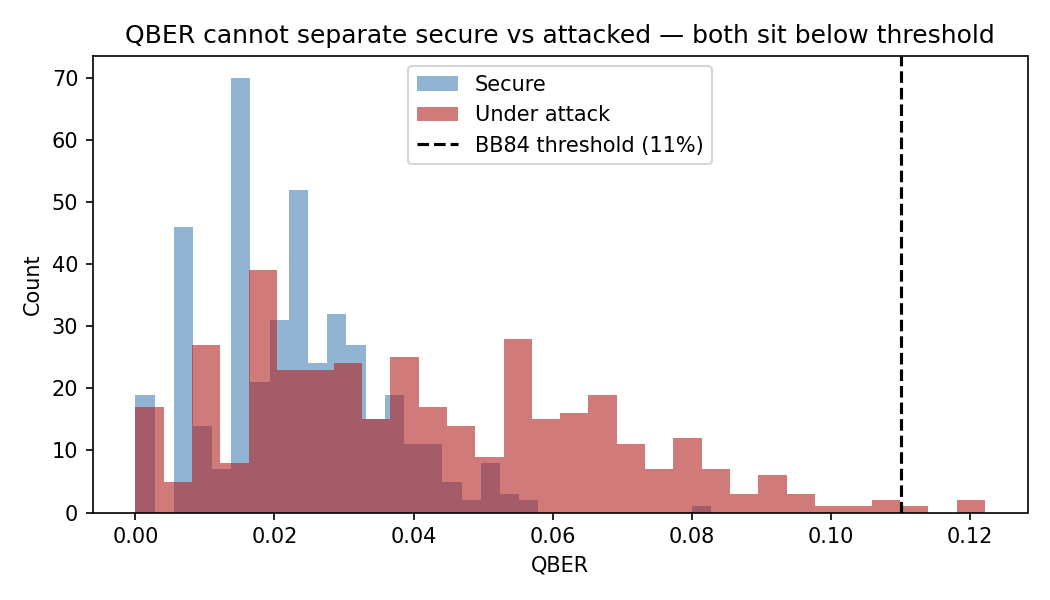
\includegraphics[width=\linewidth]{subthreshold_qber.png}\end{subfigure}\hfill
  \begin{subfigure}{0.32\textwidth}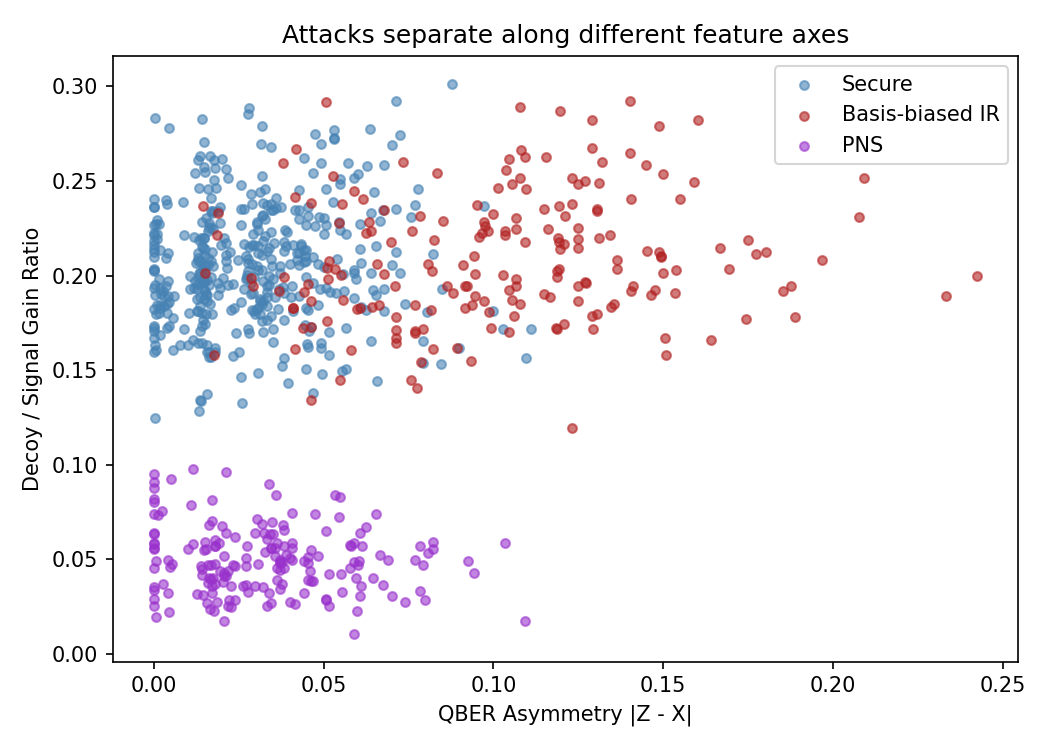
\includegraphics[width=\linewidth]{feature_separation.png}\end{subfigure}\hfill
  \begin{subfigure}{0.32\textwidth}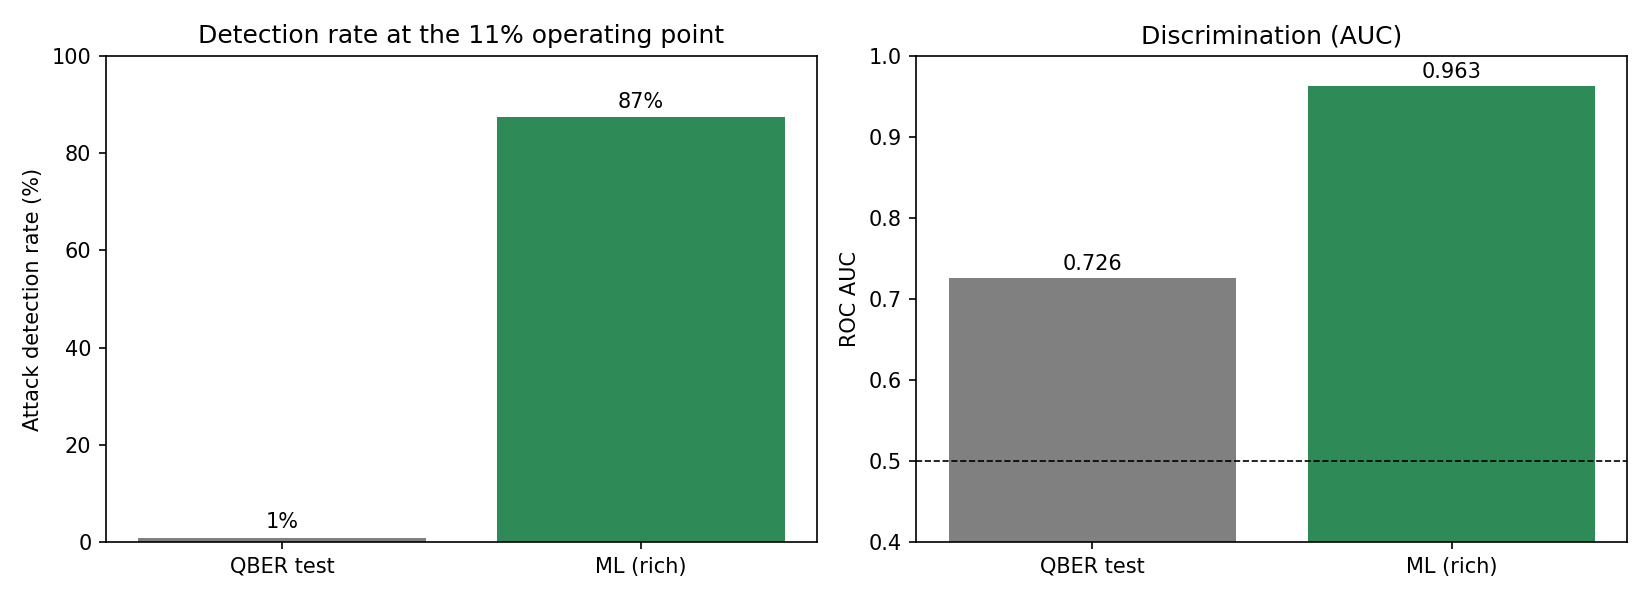
\includegraphics[width=\linewidth]{threshold_vs_ml.png}\end{subfigure}
  \caption{Sub-threshold regime: overlapping QBER (left); attacks separate in
  (asymmetry, decoy-ratio) (middle); QBER test vs ML (right).}
  \label{fig:sub}
\end{figure}

\subsection{Per-attack and classical baselines}
\begin{table}[h]
  \centering
  \caption{Per-attack discrimination and classical cross-validated AUC.}
  \begin{tabular}{lcc@{\hskip 2cm}lc}
    \toprule
    Attack & QBER-only & ML & Classifier & CV AUC \\ \midrule
    Basis-biased IR & 0.931 & 0.930 & Logistic Reg. & $0.954\pm0.012$ \\
    Gain-matched PNS & 0.508 & 1.000 & Random Forest & $0.963\pm0.008$ \\
                     &       &       & SVM           & $0.956\pm0.013$ \\
    \bottomrule
  \end{tabular}
\end{table}
PNS is invisible to QBER (AUC $0.508$, random) but perfectly detected via the decoy
ratio (AUC $1.000$).

\subsection{Classical vs.\ quantum, and kernel concentration}
On an identical $n{=}150$ set: Logistic $0.940$, SVM $0.965$, RF $0.961$, and the
\emph{tuned} quantum-kernel SVM $0.950\pm0.003$. The \emph{naive} quantum kernel
collapses to $0.577$; tuning the encoding restores $0.950$ (Figs.~\ref{fig:q}).
No quantum advantage, but no fatal disadvantage once concentration is avoided.

\begin{figure}[h]
  \centering
  \begin{subfigure}{0.33\textwidth}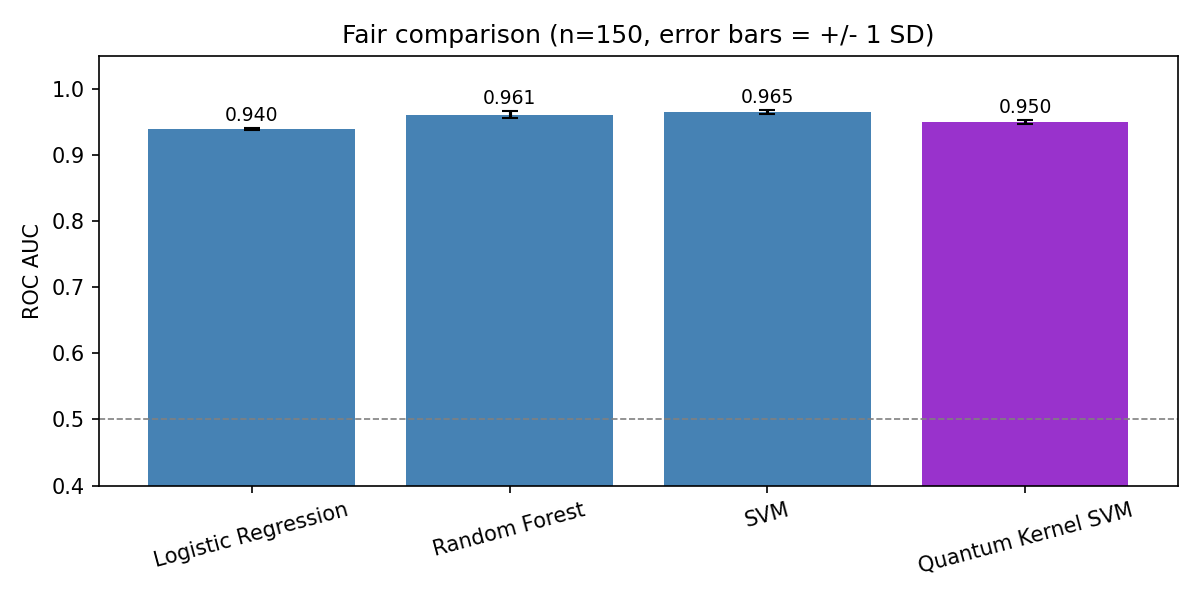
\includegraphics[width=\linewidth]{fair_comparison.png}\end{subfigure}\hfill
  \begin{subfigure}{0.33\textwidth}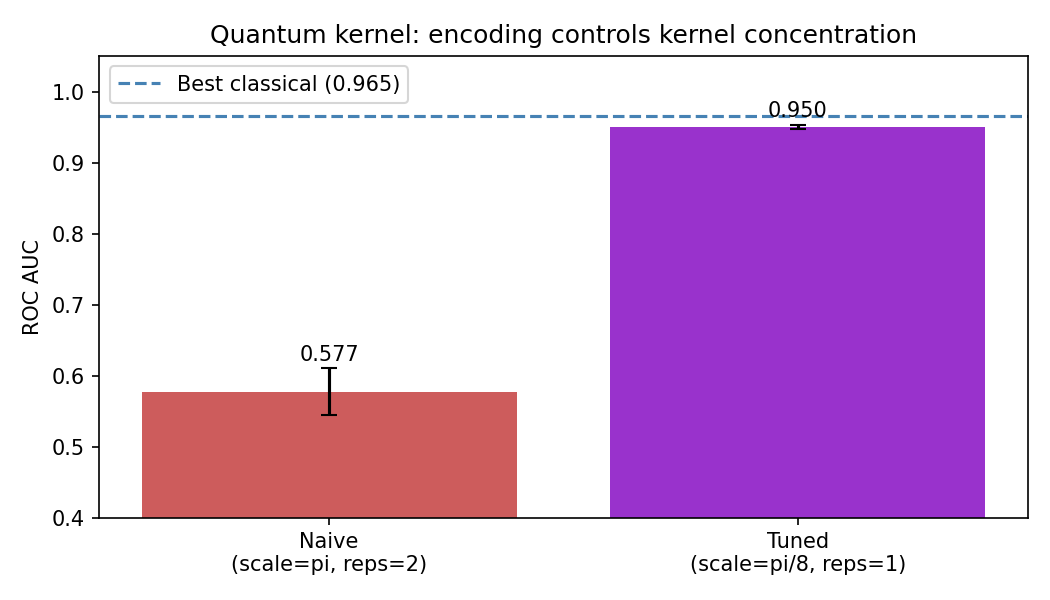
\includegraphics[width=\linewidth]{quantum_tuning.png}\end{subfigure}\hfill
  \begin{subfigure}{0.30\textwidth}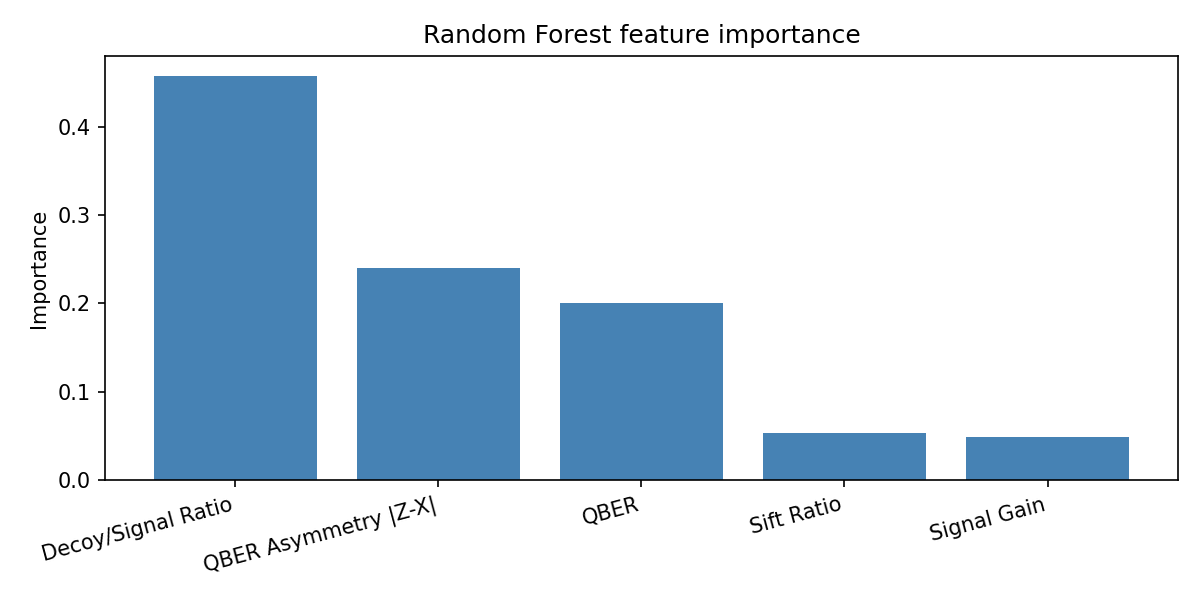
\includegraphics[width=\linewidth]{feature_importance.png}\end{subfigure}
  \caption{Fair classical/quantum comparison; encoding controls concentration
  ($0.58\!\to\!0.95$); RF feature importance (asymmetry and decoy ratio dominate).}
  \label{fig:q}
\end{figure}

\subsection{Temporal attacks}
Continuous vs bursty IR at matched mean QBER ($0.094$ vs $0.096$): the scalar
mean-QBER detector is at chance (AUC $0.559$); hand-crafted temporal features reach
$0.937$; the 1D-CNN on the raw sequence reaches $0.958$ (Figs.~\ref{fig:temp}).

\begin{figure}[h]
  \centering
  \begin{subfigure}{0.55\textwidth}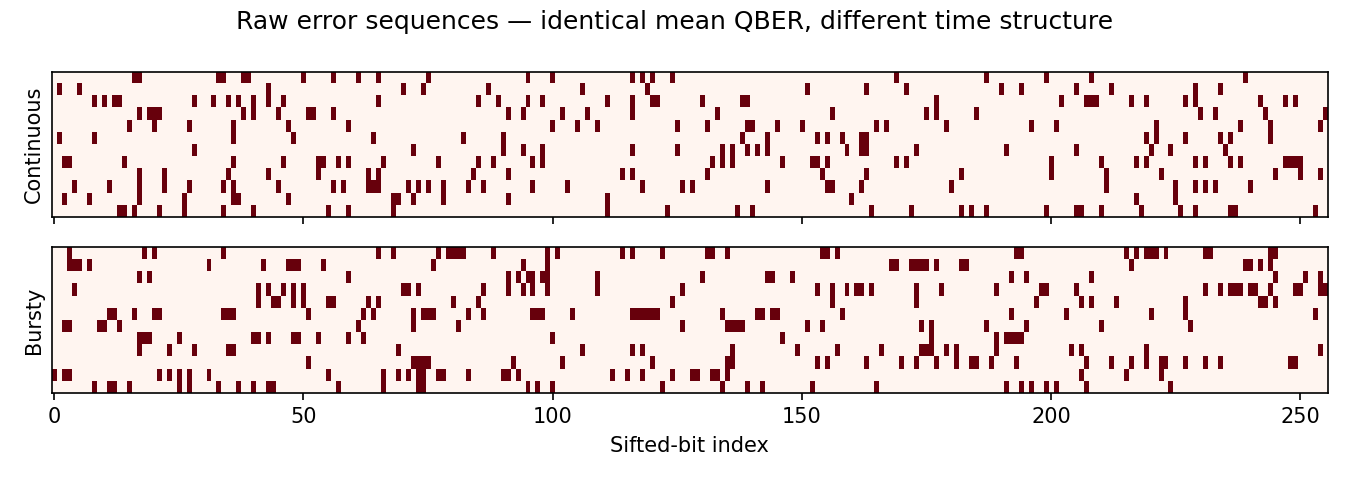
\includegraphics[width=\linewidth]{temporal_examples.png}\end{subfigure}\hfill
  \begin{subfigure}{0.42\textwidth}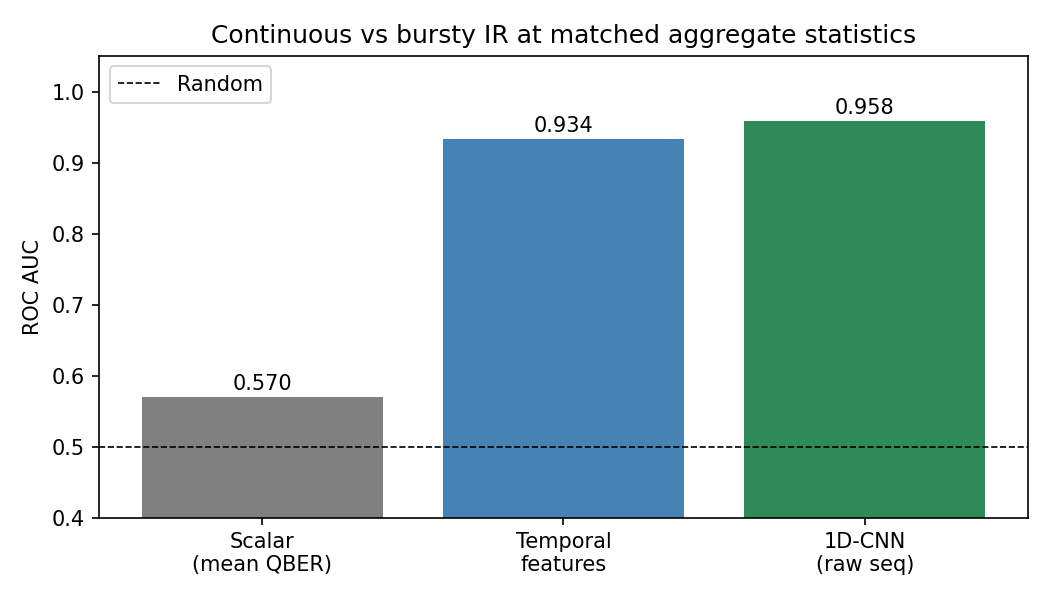
\includegraphics[width=\linewidth]{temporal_detection.png}\end{subfigure}
  \caption{Raw error sequences (same mean QBER, different clustering) and detection
  AUC by model.}
  \label{fig:temp}
\end{figure}

\section{Current status and honest novelty assessment}\label{sec:status}
\paragraph{What is built and verified.} A theory-validated BB84 simulator (photon /
decoy / depolarizing), three attack families (biased IR, gain-matched PNS,
continuous/bursty IR), two datasets, classical + quantum-kernel + 1D-CNN detectors,
full evaluation, and reproducible figures. Several real issues were found and fixed
(state-prep gate order; kernel concentration; an unphysical non-gain-matched PNS;
non-reproducible sampling; an $O(n^2)$ kernel and a per-pulse simulator, both
optimized).

\paragraph{Novelty --- candid.} None of the results is a new scientific
\emph{discovery}. ML-for-QKD detection, decoy-state PNS detection, per-basis
asymmetry, quantum-kernel concentration, the adaptive-eavesdropper game, and the
finite-key stealth floor are all established in the 2025--2026 literature --- in
particular the adaptive-attacker game with decoy-aware/temporal detectors and a
finite-key stealth floor is developed more rigorously (entropy-accumulation bounds,
more attack families) by Al-Mohammed and Al-Ali (arXiv:2603.03502), and multi-attack
DV-QKD detection with CNN/LSTM/quantum-LSTM classifiers by arXiv:2509.14282. A
literature search was run specifically to test each of our directions, and each was
found covered. The project's value is therefore \emph{reproduction, validation, and
honest positioning}, not discovery.

\paragraph{Adaptive-attacker coverage study (\texttt{src/adversarial/}).} We study
detection as a game where Eve chooses an attack policy over a channel palette
(intercept--resend, basis-biased IR, gain-matched PNS) on a shared information axis
$I$ = fraction of the sifted key she learns, and measure her \emph{best response}
against four detectors of increasing feature coverage at a $5\%$ false-alarm rate.
We reproduce a two-regime characterization:
\begin{itemize}
  \item \textbf{Coverage failure:} QBER-only and asymmetry-aware detectors are
  evaded at \emph{every} $I$ (detection $\approx$ the $5\%$ floor) --- Eve switches
  to PNS, whose signature they do not measure. Qualitative; unfixable by more data.
  \item \textbf{Finite-key stealth floor:} decoy-aware/combined detectors catch
  PNS, with detection rising in $I$; the low-$I$ gap is purely finite-sample ---
  at fixed $I\!\approx\!0.37$, combined detection rises $0.14\to0.64\to0.96$ as the
  key grows from 2k to 20k pulses.
\end{itemize}
Signature-splitting (IR/PNS mixes) does not help Eve; pure PNS is her dominant
evasion. These effects are consistent with arXiv:2603.03502; we reproduce them
independently on a single transparent, theory-validated testbed. ``Adversarial''
here means an adaptive eavesdropper choosing a physical attack strategy --- distinct
from input-perturbation adversarial \emph{examples} on quantum classifiers.

\begin{thebibliography}{9}
\bibitem{bb84} C.~H.~Bennett, G.~Brassard, \emph{Proc.\ IEEE ICCSSP}, 1984.
\bibitem{shorpreskill} P.~W.~Shor, J.~Preskill, \emph{Phys.\ Rev.\ Lett.} \textbf{85}, 441 (2000).
\bibitem{decoy} H.-K.~Lo, X.~Ma, K.~Chen, \emph{Phys.\ Rev.\ Lett.} \textbf{94}, 230504 (2005).
\bibitem{concentration} S.~Thanasilp et al., ``Exponential concentration in quantum kernel methods,'' 2022.
\end{thebibliography}

\end{document}
